\section{Examples of Elementary Systems; Applications}

\paragraph{\textbf{5.1.}}
\SGARefTarget{sga3:xx:5.1}
Let \(S\) be a scheme and \(L\) an invertible
\(\mathcal O_S\)-module.  Consider the group \(\mathrm{GL}_L\) over
\(S\) defined by
\[
 \mathrm{GL}_L(S')
 =
 \left\{
 \begin{pmatrix}a&b\\c&d\end{pmatrix}
 \ \middle|\
 \begin{array}{l}
 a,d\in\mathbb G_a(S'),\quad b\in W(L)(S'),\\
 c\in W(L^{-1})(S'),\quad ad-bc\in\mathbb G_m(S')
 \end{array}
 \right\},
\]
equipped with the usual matrix-multiplication law.  It is locally
isomorphic to \(\mathrm{GL}_{2,S}\).  It is therefore an affine smooth
\(S\)-group scheme with connected fibers.

\smallskip
\noindent\textit{Remark.}
Let \(L'\) and \(L''\) be invertible sheaves on \(S\) such that
\[
 L=L'\otimes L''^{-1}.
\]
Then there is an isomorphism of \(S\)-groups
\[
 \mathrm{GL}_L\xrightarrow{\ \sim\ }\mathrm{GL}(L'\oplus L'')
\]
defined as follows: if \(x\) (respectively \(y\)) is a section of
\(L'\) (respectively \(L''\)) on an open subset \(V\) of \(S\), then
\[
 \begin{pmatrix}a&b\\c&d\end{pmatrix}
 \begin{pmatrix}x\\y\end{pmatrix}
 =
 \begin{pmatrix}ax+by\\cx+dy\end{pmatrix}.
\]
\footnote{The editors corrected
\(L''\otimes L'^{-1}\) to \(L'\otimes L''^{-1}\) and expanded the
sentence that follows.}

\paragraph{\textbf{5.2.}}
\SGARefTarget{sga3:xx:5.2}
Denote by \(\mathrm{SL}_L\) the closed subgroup of
\(\mathrm{GL}_L\) defined by \(ad-bc=1\).  It too is an affine smooth
\(S\)-group scheme with connected fibers; under the preceding
isomorphism it is isomorphic to \(\mathrm{SL}(L'\oplus L'')\).

Likewise, consider the morphism
\[
 \mathbb G_{m,S}\longrightarrow\mathrm{GL}_L,
 \qquad
 z\longmapsto\begin{pmatrix}z&0\\0&z\end{pmatrix}.
\]
It is a central monomorphism.  Passage to the quotient gives a smooth
affine \(S\)-group \(\mathrm P_L\) with connected fibers
\textup{(cf.\ \SGARefLink{sga3:viii:corollary:5:7}{Exposé VIII, 5.7})}.  By passing to the quotient in the
isomorphism of the preceding remark, one sees that \(\mathrm P_L\)
identifies with the automorphism group of the projective bundle
\(\mathbb P(L'\oplus L'')\) \textup{(cf.\ EGA II, 4.2.7)}.
Write \(i\) and \(p\) for the canonical morphisms
\[
 \mathrm{SL}_L\xrightarrow{\ i\ }\mathrm{GL}_L
   \xrightarrow{\ p\ }\mathrm P_L.
\]
Here \(i\) is a closed immersion, while \(p\) is faithfully flat and
affine.

\paragraph{\textbf{5.3.}}
\SGARefTarget{sga3:xx:5.3}
Consider the group morphisms
\[
\begin{aligned}
 t_G\colon\mathbb G_{m,S}^{\,2}&\longrightarrow\mathrm{GL}_L,
 &t_G(z,z')&=\begin{pmatrix}z&0\\0&z'\end{pmatrix},\\
 t_S\colon\mathbb G_{m,S}&\longrightarrow\mathrm{SL}_L,
 &t_S(z)&=\begin{pmatrix}z&0\\0&z^{-1}\end{pmatrix},\\
 t_P\colon\mathbb G_{m,S}&\longrightarrow\mathrm P_L,
 &t_P(z)&=p\bigl(t_G(z,1)\bigr).
\end{aligned}
\]
They are group monomorphisms and define in each group a split torus of
relative codimension \(2\).  For \(s\in S\), let
\[
 X\in\Gamma(s,L\otimes s)^\times.
\]
The section
\(\begin{psmallmatrix}0&X\\-X^{-1}&0\end{psmallmatrix}\) of
\(\mathrm{GL}_{L,s}\) normalizes \(t_G(\mathbb G_{m,s}^{\,2})\) and
does not centralize it.  \SGARefLink{sga3:xix:definition:1:6:1}{Exposé XIX, 1.6} therefore shows that
\(\mathrm{GL}_L\) is reductive of semisimple rank \(1\), with maximal
torus \(t_G(\mathbb G_{m,S}^{\,2})\).  The same argument shows that
\(\mathrm{SL}_L\) and \(\mathrm P_L\) are reductive of semisimple rank
\(1\), with respective maximal tori
\(t_S(\mathbb G_{m,S})\) and \(t_P(\mathbb G_{m,S})\).

\paragraph{\textbf{5.4.}}
\SGARefTarget{sga3:xx:5.4}
The Lie algebras of these groups, and the adjoint actions of the
chosen maximal tori, are determined in the usual way.  For
\(\mathrm{GL}_L\), \SGARefLink{sga3:ii:proposition:4-8}{Exposé II, 4.8} immediately gives
\[
 \Lie(\mathrm{GL}_L/S)
 =
 \left\{
 \begin{pmatrix}a&b\\c&d\end{pmatrix}
 \ \middle|\
 a,d\in\mathcal O_S,\ b\in L,\ c\in L^{-1}
 \right\},
\]
with the usual bracket, and
\[
 \operatorname{Ad}\bigl(t_G(z,z')\bigr)
 \begin{pmatrix}a&b\\c&d\end{pmatrix}
 =
 \begin{pmatrix}
 a&zz'^{-1}b\\
 z'z^{-1}c&d
 \end{pmatrix}.
\]
Put \(\mathfrak g=\Lie(\mathrm{GL}_L/S)\), and define
\[
 \alpha_G\colon t_G(\mathbb G_{m,S}^{\,2})\longrightarrow
 \mathbb G_{m,S},
 \qquad
 \alpha_G\bigl(t_G(z,z')\bigr)=zz'^{-1}.
\]
The preceding identity shows that \(\alpha_G\) is a root of
\(\mathrm{GL}_L\) relative to \(t_G(\mathbb G_{m,S}^{\,2})\), and
that
\[
 u\colon L\longrightarrow\mathfrak g,
 \quad X\longmapsto\begin{pmatrix}0&X\\0&0\end{pmatrix},
 \qquad
 u^-\colon L^{-1}\longrightarrow\mathfrak g,
 \quad Y\longmapsto\begin{pmatrix}0&0\\Y&0\end{pmatrix}
\]
identify \(L\) with \(\mathfrak g^{\alpha_G}\) and \(L^{-1}\) with
\(\mathfrak g^{-\alpha_G}\), respectively.  Thus
\[
 \bigl(\mathrm{GL}_L,t_G(\mathbb G_{m,S}^{\,2}),\alpha_G\bigr)
\]
is an elementary \(S\)-system.

Similarly, setting
\[
 \alpha_S(t_S(z))=z^2,
 \qquad
 \alpha_P(t_P(z))=z,
\]
one finds elementary \(S\)-systems
\[
 \bigl(\mathrm{SL}_L,t_S(\mathbb G_{m,S}),\alpha_S\bigr),
 \qquad
 \bigl(\mathrm P_L,t_P(\mathbb G_{m,S}),\alpha_P\bigr),
\]
and corresponding identifications of \(L\) and \(L^{-1}\) with the
root summands of their Lie algebras.

\paragraph{\textbf{5.5.}}
\SGARefTarget{sga3:xx:5.5}
Set
\[
 \exp\begin{pmatrix}0&X\\0&0\end{pmatrix}
   =\begin{pmatrix}1&X\\0&1\end{pmatrix}.
\]
This defines a morphism
\[
 W(\mathfrak g^{\alpha_G})\longrightarrow\mathrm{GL}_L
\]
whose tangent map is the canonical inclusion; it is therefore the
unique morphism of this kind by \SGARefLink{sga3:xx:1.5}{1.5}.  Likewise, set
\[
 \exp\begin{pmatrix}0&0\\Y&0\end{pmatrix}
   =\begin{pmatrix}1&0\\Y&1\end{pmatrix}.
\]
Direct calculation of formula \textup{(F)} gives
\[
 \left\langle
 \begin{pmatrix}0&X\\0&0\end{pmatrix},
 \begin{pmatrix}0&0\\Y&0\end{pmatrix}
 \right\rangle
 =XY,
 \qquad
 \alpha_G^\ast(z)
 =\begin{pmatrix}z&0\\0&z^{-1}\end{pmatrix}
 =t_G(z,z^{-1}).
\]
\footnote{The editors expanded the calculations that follow.}

The open subset \(N^\times=N_G^\times\) defined before \SGARefLink{sga3:xx:3.1}{3.1} is
\[
 N_G^\times(S')
 =
 \left\{
 \begin{pmatrix}0&P\\Q&0\end{pmatrix}
 \ \middle|\
 P\in W(\mathfrak g^\alpha)^\times(S'),\
 Q\in W(\mathfrak g^{-\alpha})^\times(S')
 \right\}.
\]
For \(X\in W(\mathfrak g^\alpha)^\times(S')\),
\[
 w_{\alpha_G}(X)
 =\begin{pmatrix}0&X\\-X^{-1}&0\end{pmatrix}.
\]
Moreover, if
\[
 w=\begin{pmatrix}0&P\\Q&0\end{pmatrix}\in N_G^\times(S'),
\]
then
\[
 a_{\alpha_G}(w)=PQ^{-1}
   \in W\bigl((\mathfrak g^\alpha)^{\otimes2}\bigr)^\times(S');
\]
that is, for \(Y\in W(\mathfrak g^{-\alpha})^\times(S')\),
\[
 a_{\alpha_G}(w)(Y)=PQ^{-1}Y
   \in W(\mathfrak g^\alpha)^\times(S').
\]

\paragraph{\textbf{5.6.}}
\SGARefTarget{sga3:xx:5.6}
We leave the analogous calculations for \(\mathrm{SL}_L\) and
\(\mathrm P_L\) to the reader.  One obtains the same duality formula
and the coroots
\[
 \alpha_S^\ast(z)=t_S(z),
 \qquad
 \alpha_P^\ast(z)=t_P(z^2).
\]
Let \(p_T\) be the morphism induced by
\(p\colon\mathrm{GL}_L\to\mathrm P_L\) on
\(t_S(\mathbb G_{m,S})\), namely
\[
 p_T(t_S(z))=t_P(z^2).
\]
Thus the following diagram is commutative:
\footnote{Here \(t_S\) and \(t_P\) are isomorphisms.}
\begin{center}
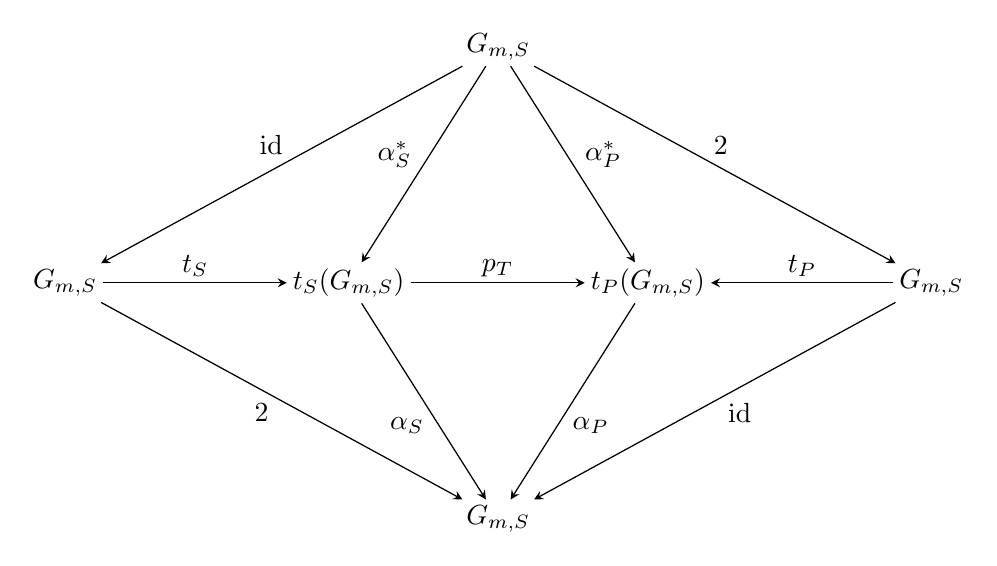
\begin{tikzpicture}[>=stealth,
  every node/.style={inner sep=2pt},
  every path/.style={line width=.45pt}]
  \node (top) at (0,3.0) {$\mathbb G_{m,S}$};
  \node (left) at (-5.5,0) {$\mathbb G_{m,S}$};
  \node (ts) at (-1.9,0) {$t_S(\mathbb G_{m,S})$};
  \node (tp) at (1.9,0) {$t_P(\mathbb G_{m,S})$};
  \node (right) at (5.5,0) {$\mathbb G_{m,S}$};
  \node (bottom) at (0,-3.0) {$\mathbb G_{m,S}$};

  \draw[->] (top) -- node[pos=.48,above left] {$\mathrm{id}$} (left);
  \draw[->] (top) -- node[pos=.55,above left] {$\alpha_S^\ast$} (ts);
  \draw[->] (top) -- node[pos=.55,above right] {$\alpha_P^\ast$} (tp);
  \draw[->] (top) -- node[pos=.48,above right] {$2$} (right);

  \draw[->] (left) -- node[above] {$t_S$} (ts);
  \draw[->] (ts) -- node[above] {$p_T$} (tp);
  \draw[->] (right) -- node[above] {$t_P$} (tp);

  \draw[->] (left) -- node[pos=.48,below left] {$2$} (bottom);
  \draw[->] (ts) -- node[pos=.55,below left] {$\alpha_S$} (bottom);
  \draw[->] (tp) -- node[pos=.55,below right] {$\alpha_P$} (bottom);
  \draw[->] (right) -- node[pos=.48,below right] {$\mathrm{id}$} (bottom);
\end{tikzpicture}
\end{center}
Its central portion is the commutative diagram of \SGARefLink{sga3:xx:4.1}{4.1}
\footnote{With \(q=1\).}
associated with the canonical morphism
\(p\circ i\colon\mathrm{SL}_L\to\mathrm P_L\), which induces a
morphism between the preceding elementary \(S\)-systems.

